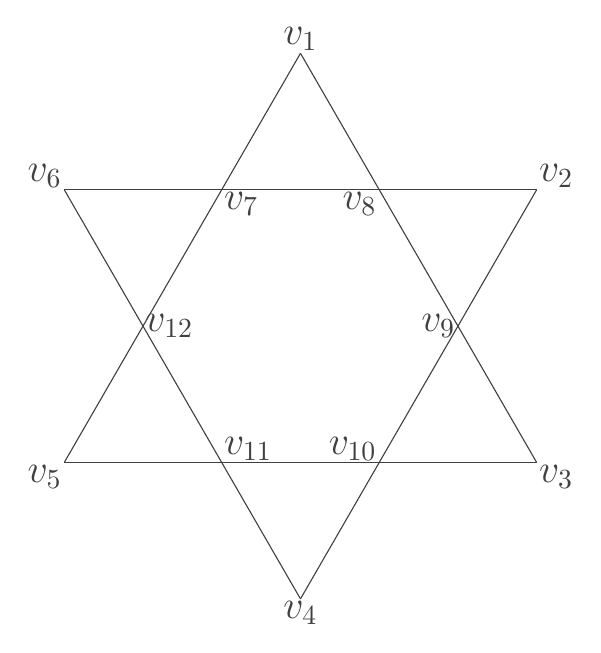
\begin{tikzpicture}[draw=darkgray, text=darkgray, align=center, xscale=1, yscale=sqrt(3)/2, scale=2]
    \tikzstyle{every node}=[inner sep=0pt];

    \node at ( 0.0,  2)  (a) [label=above:{\Large$v_{1}$}] {};
    \node at (-1.5,  1)  (b) [label=above left:{\Large$v_{6}$}] {};
    \node at (-0.5,  1)  (c) [label=below right:{\Large$v_{7}$}] {};
    \node at ( 0.5,  1)  (d) [label=below left:{\Large$v_{8}$}] {};
    \node at ( 1.5,  1)  (e) [label=above right:{\Large$v_{2}$}] {};
    \node at (-1.0,  0)  (f) [label=right:{\Large$v_{12}$}] {};
    \node at ( 1.0,  0)  (g) [label=left:{\Large$v_{9}$}] {};
    \node at (-1.5, -1)  (h) [label=below left:{\Large$v_{5}$}] {};
    \node at (-0.5, -1)  (i) [label=above right:{\Large$v_{11}$}] {};
    \node at ( 0.5, -1)  (j) [label=above left:{\Large$v_{10}$}] {};
    \node at ( 1.5, -1)  (k) [label=below right:{\Large$v_{3}$}] {};
    \node at ( 0.0, -2)  (l) [label=below:{\Large$v_{4}$}] {};

    \path (c.center)
        edge (a.center)
        edge (b.center)
        edge (d.center);
    \path (d.center)
        edge (a.center)
        edge (e.center)
        edge (g.center);
    \path (g.center)
        edge (e.center)
        edge (k.center)
        edge (j.center);
    \path (j.center)
        edge (k.center)
        edge (l.center)
        edge (i.center);
    \path (i.center)
        edge (l.center)
        edge (h.center)
        edge (f.center);
    \path (f.center)
        edge (h.center)
        edge (b.center)
        edge (c.center);
\end{tikzpicture}
